\section{Implémentation}
\section{GrapheDBJ}
Le passage du graphe de De Bruijn aux contigs finaux dans ce code s'opère en trois phases distinctes : la simplification topologique, la traversée pour la génération de séquences brutes, et enfin une étape de fusion (Overlap-Layout-Consensus) pour assembler les fragments restants.

\subsection{Simplification Préalable du Graphe}
Avant de tenter de générer des contigs, le programme nettoie le graphe pour éliminer les artefacts de séquençage. Cette étape est orchestrée dans le fichier \texttt{main.cpp} via une boucle itérative qui appelle séquentiellement deux fonctions de la classe \texttt{GraphDBJ} jusqu'à stabilisation ou atteinte du nombre maximal de passes \texttt{max\_passes\_pop}.


\subsubsection{Suppression des Pointes (Tips)}
La méthode \texttt{clipTips()} parcourt la \texttt{nodes\_map} pour identifier les nœuds sans enfants (culs-de-sac). Elle remonte le chemin inverse pour vérifier la longueur de la branche morte. Si la longueur est inférieure à \texttt{TOPO\_MAX\_LEN} ou si la couverture est trop faible par rapport à l'ancrage (ratio défini par \texttt{RCTC\_RATIO}), la branche est coupée via \texttt{disconnectNodes} et les nœuds marqués \texttt{removed = true}.


\subsubsection{Résolution des Bulles}
La méthode \texttt{resolveBubbles()} détecte les divergences où un nœud possède exactement deux enfants qui finissent par converger vers un ancêtre commun plus loin (profondeur limitée par \texttt{SEARCH\_DEPTH\_FACTOR}). L'algorithme compare la couverture cumulée des deux chemins (le chemin "gagnant" est celui avec la plus haute couverture) et marque logiquement les nœuds du chemin perdant comme supprimés.

\subsection{Génération des Contigs Bruts}
Une fois le graphe nettoyé, la fonction \texttt{GraphDBJ::generateContigs()} est invoquée pour transformer les chemins de graphe en séquences linéaires.


\begin{itemize}
    \item \textbf{Identification des points de départ :} L'algorithme itère sur tous les nœuds et initie un nouveau contig si un nœud est un début potentiel (pas de parents) ou un point de jonction complexe (plusieurs parents).
    \item \textbf{Traversée gloutonne :} À partir du nœud de départ, une boucle \texttt{while} suit les arêtes sortantes.
    \begin{itemize}
        \item Si le nœud courant a un seul enfant, l'extension est triviale.
        \item En cas de bifurcation (plusieurs enfants), l'algorithme utilise une heuristique de couverture : il sélectionne l'enfant ayant la couverture maximale si celle-ci est supérieure à celle du second meilleur enfant multipliée par \texttt{COVERAGE\_RATIO}.
    \end{itemize}
    \item \textbf{Construction de la séquence :} Les nucléotides sont extraits des nœuds et ajoutés progressivement à un objet \texttt{BitVector} représentant le contig en cours de construction.
\end{itemize}

\subsection{Fusion des Contigs (Post-traitement)}
La fonction \texttt{mergeContigs} agit comme le « cerveau » du post-traitement de l'assembleur GraphDBJ. Son objectif principal est de recoudre les contigs fragmentés qui n'ont pas pu être fusionnés lors du parcours du graphe en raison d'erreurs de séquençage ou d'une topologie complexe.

Contrairement aux assembleurs standards qui n'inspectent que les extrémités immédiates (les pointes) des contigs, cette implémentation utilise une stratégie de \textbf{« Deep Seeding » (Ensemencement Profond)} couplée à un mécanisme d'\textbf{Extension Bidirectionnelle}.

\usetikzlibrary{shapes.geometric, arrows, positioning, calc, fit, backgrounds}

\tikzset{
    startstop/.style={rectangle, rounded corners, minimum width=3cm, minimum height=1cm, text centered, draw=black, fill=blue!10},
    process/.style={rectangle, minimum width=3cm, minimum height=1cm, text centered, draw=black, fill=green!10},
    decision/.style={diamond, aspect=2, minimum width=3cm, minimum height=1cm, text centered, draw=black, fill=orange!10},
    arrow/.style={thick,->,>=stealth'},
    block/.style={rectangle, minimum width=3cm, minimum height=1cm, text width=5cm, text centered, draw=black, fill=gray!10},
    substep/.style={rectangle, minimum width=2.5cm, minimum height=0.8cm, text width=5cm, align=center, draw=black!50, fill=white},
    % Nouveaux styles pour les cadres de fond
    phasebox/.style={draw, dashed, rounded corners, inner sep=0.5cm, line width=1pt}
}

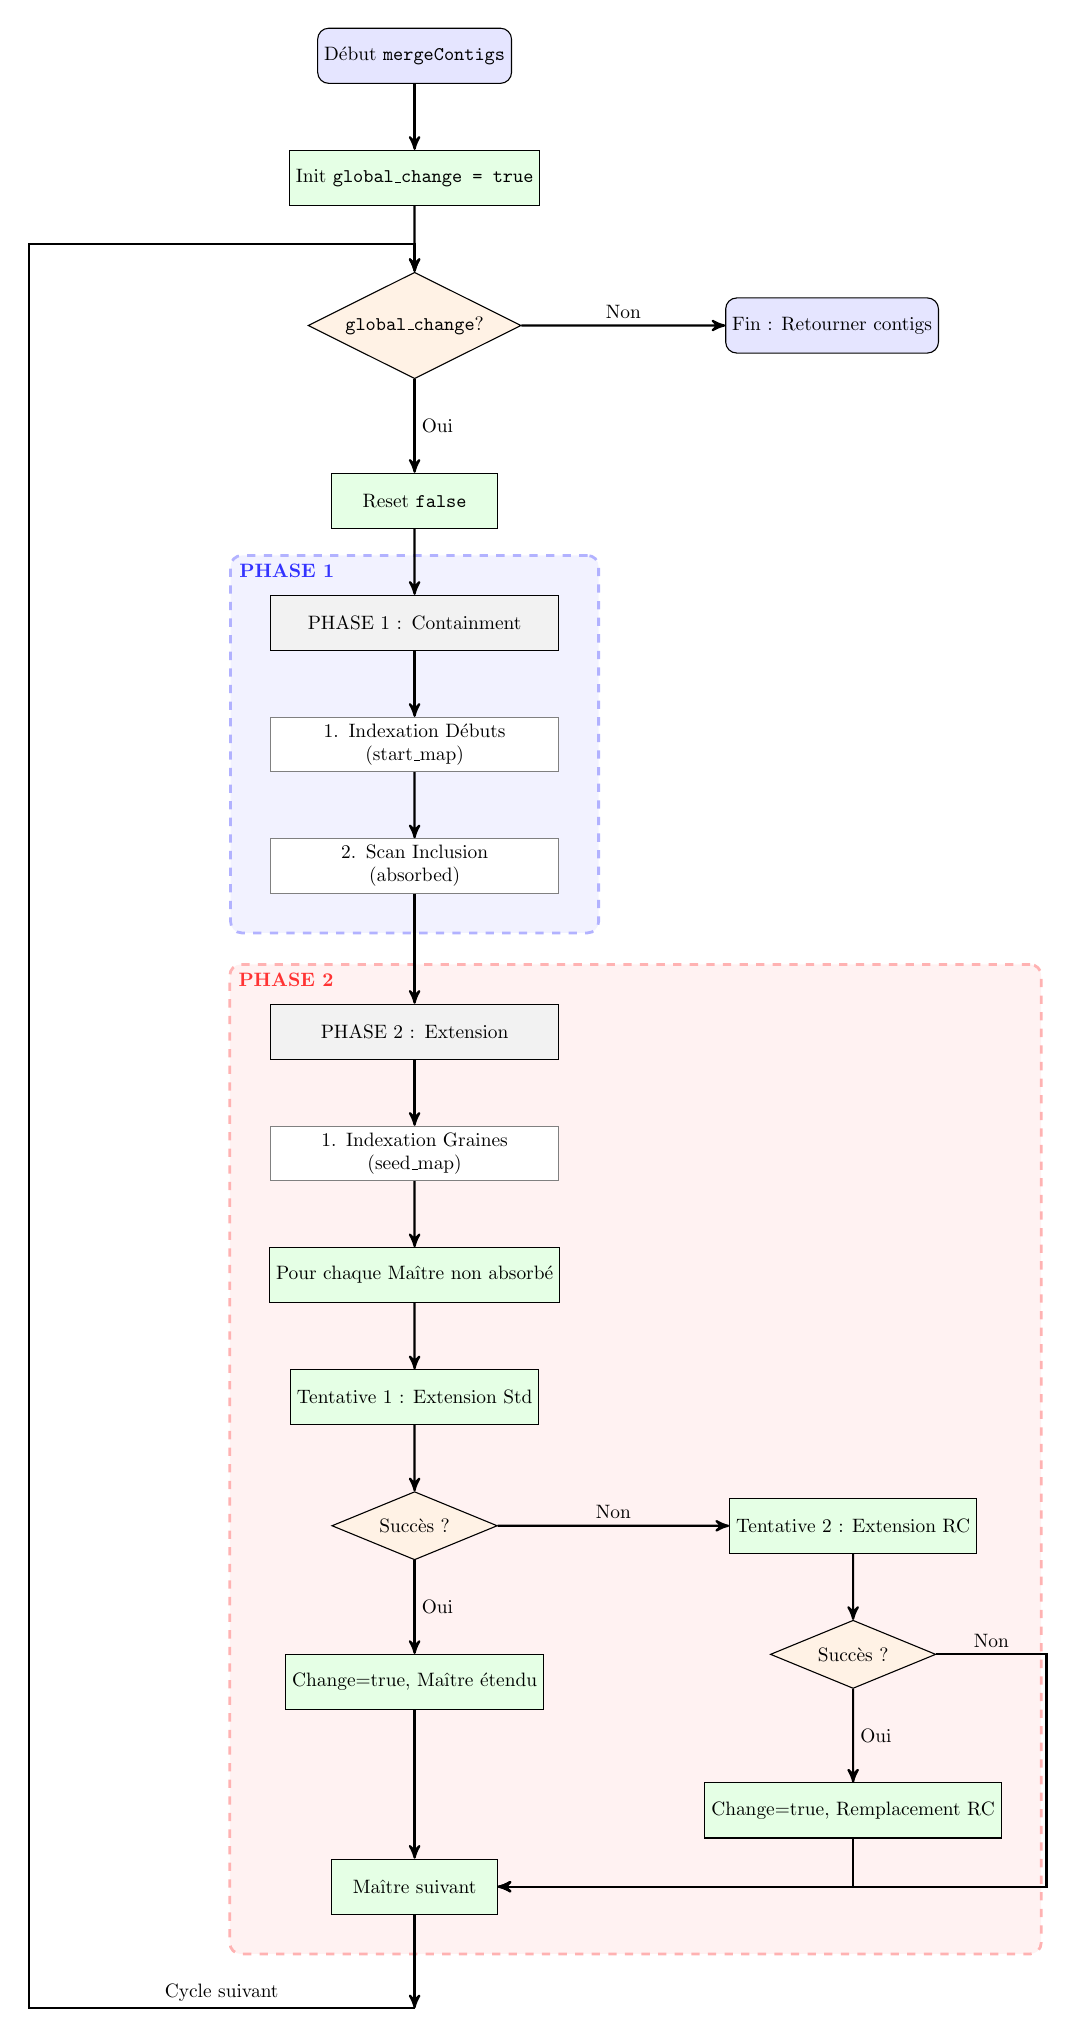
\begin{tikzpicture}[node distance=1.2cm, auto, scale=0.7, transform shape]

    % --- NOEUDS ---
    \node (start) [startstop] {Début \texttt{mergeContigs}};
    \node (global_loop_init) [process, below=of start] {Init \texttt{global\_change = true}};
    \node (global_loop_decision) [decision, below=of global_loop_init] {\texttt{global\_change}?};
    \node (end) [startstop, right=of global_loop_decision, xshift=2.5cm] {Fin : Retourner contigs};
    \node (global_loop_reset) [process, below=of global_loop_decision, yshift=-0.5cm] {Reset \texttt{false}};

    % --- PHASE 1 ---
    \node (phase1_label) [block, below=of global_loop_reset] {PHASE 1 : Containment};
    \node (phase1_step1) [substep, below=of phase1_label] {1. Indexation Débuts\\ (start\_map)};
    \node (phase1_step2) [substep, below=of phase1_step1] {2. Scan Inclusion\\ (absorbed)};
    
    % --- PHASE 2 ---
    \node (phase2_label) [block, below=of phase1_step2, yshift=-0.8cm] {PHASE 2 : Extension};
    \node (phase2_step1) [substep, below=of phase2_label] {1. Indexation Graines\\ (seed\_map)};
    \node (phase2_loop_start) [process, below=of phase2_step1] {Pour chaque Maître non absorbé};
    
    \node (try_std_ext) [process, below=of phase2_loop_start] {Tentative 1 : Extension Std};
    \node (std_ext_success) [decision, below=of try_std_ext] {Succès ?};
    \node (merge_success_std) [process, below=of std_ext_success, yshift=-0.5cm] {Change=true, Maître étendu};

    \node (try_rc_ext) [process, right=of std_ext_success, xshift=3cm] {Tentative 2 : Extension RC};
    \node (rc_ext_success) [decision, below=of try_rc_ext] {Succès ?};
    \node (merge_success_rc) [process, below=of rc_ext_success, yshift=-0.5cm] {Change=true, Remplacement RC};

    \node (next_master) [process, below=of merge_success_std, yshift=-1.5cm] {Maître suivant};
    \node (end_loop_phase2) [coordinate, below=of next_master, yshift=-0.5cm] {};

    % --- FLÈCHES ---
    \draw [arrow] (start) -- (global_loop_init);
    \draw [arrow] (global_loop_init) -- (global_loop_decision);
    \draw [arrow] (global_loop_decision) -- node[above] {Non} (end);
    \draw [arrow] (global_loop_decision) -- node[right] {Oui} (global_loop_reset);
    \draw [arrow] (global_loop_reset) -- (phase1_label);
    \draw [arrow] (phase1_label) -- (phase1_step1);
    \draw [arrow] (phase1_step1) -- (phase1_step2);
    \draw [arrow] (phase1_step2) -- (phase2_label);
    \draw [arrow] (phase2_label) -- (phase2_step1);
    \draw [arrow] (phase2_step1) -- (phase2_loop_start);
    \draw [arrow] (phase2_loop_start) -- (try_std_ext);
    \draw [arrow] (try_std_ext) -- (std_ext_success);
    
    \draw [arrow] (std_ext_success) -- node[right] {Oui} (merge_success_std);
    \draw [arrow] (std_ext_success) -- node[above] {Non} (try_rc_ext);
    
    \draw [arrow] (try_rc_ext) -- (rc_ext_success);
    \draw [arrow] (rc_ext_success) -- node[right] {Oui} (merge_success_rc);
    
    % Flèche NON qui contourne large
    \draw [arrow] (rc_ext_success.east) -- node[above] {Non} ++(2,0) |- (next_master.east);

    \draw [arrow] (merge_success_std) -- (next_master);
    \draw [arrow] (merge_success_rc.south) |- (next_master);

    \draw [arrow] (next_master) -- (end_loop_phase2);
    \draw [arrow] (end_loop_phase2) -- ++(-7,0) node[midway, above] {Cycle suivant} |- ([yshift=0.5cm]global_loop_decision.north) -- (global_loop_decision.north);

    % --- CADRES DE FOND (BACKGROUNDS) ---
    % On utilise un layer pour dessiner DERRIÈRE les noeuds existants
    \begin{pgfonlayer}{background}
        
        % Cadre Phase 1 : Englobe le label Phase 1 et l'étape 2
        \node [fit=(phase1_label) (phase1_step2), 
               phasebox, fill=blue!5, draw=blue!30, 
               label={[anchor=north west, inner sep=5pt, color=blue!80]north west:\textbf{PHASE 1}}] {};

        % Cadre Phase 2 : Englobe le label Phase 2, l'extension RC (tout à droite) et le maitre suivant (tout en bas)
        \node [fit=(phase2_label) (try_rc_ext) (merge_success_rc) (next_master) (phase2_loop_start), 
               phasebox, fill=red!5, draw=red!30, 
               label={[anchor=north west, inner sep=5pt, color=red!80]north west:\textbf{PHASE 2}}] {};
               
    \end{pgfonlayer}

\end{tikzpicture}

\subsection{Le « Deep Seeding »}
La logique de fusion standard examine souvent uniquement les derniers $k$ nucléotides. Cette méthode est rapide mais fragile ; si les 10 dernières bases contiennent une erreur de séquençage, la fusion échoue.

Le \textbf{Deep Seeding} scanne profondément à l'intérieur du contig « Maître » (jusqu'à 5000 pb) pour trouver une correspondance avec un contig « Candidat ». Cela permet à l'algorithme de contourner les « pointes sales » (erreurs en fin de lecture) et de localiser le véritable chevauchement propre, enfoui plus profondément dans la séquence.

\subsection{Phase 1 : Containment}
Avant de fusionner, l'assembleur doit éliminer la redondance. Souvent, le graphe produit un long contig (ex: 10kpb) et une copie plus courte et redondante (ex: 500pb) qui est identique à une sous-séquence du grand contig.

\subsubsection{Indexation des Départs}
Une table de hachage (\texttt{start\_map}) est créée pour stocker le premier $k$-mer de chaque contig.
\begin{itemize}
    \item \textbf{Efficacité :} Vérifier chaque contig contre tous les autres est en $O(N^2)$. L'indexation réduit considérablement ce coût.
    \item \textbf{Complément Inverse (RC) :} Nous indexons à la fois le début \textit{Forward} (Sens) et le début \textit{RC} (Anti-sens), car un petit contig peut être orienté « à l'envers » par rapport au maître.
\end{itemize}

\subsubsection{Logique de Scan}
L'algorithme itère sur chaque contig « Maître » et scanne chaque position :

\begin{lstlisting}[language=C++, caption={Pseudo-code de la logique d'inclusion}]
// Logique simplifiee
Pour chaque position 'pos' dans Maitre :
   cle = getKmerAt(pos)
   si (cle existe dans start_map) :
       Candidat = start_map[cle]
       Verifier si le Candidat s'insere parfaitement dans le Maitre a 'pos'
       Si oui -> Marquer le Candidat comme ABSORBE (le supprimer)
\end{lstlisting}

\subsection{Phase 2 : Extension Profonde}
Cette phase joint les contigs distincts et propres. La logique est enveloppée dans une boucle \texttt{while(global\_change)}, garantissant que si la fusion de A et B crée une nouvelle queue qui correspond à C, le processus continue jusqu'à stabilisation.

\subsubsection{L'Index de Graines}
Un index (\texttt{seed\_map}) de tous les candidats disponibles est construit. Nous indexons toutes les $k$-ièmes positions (ex: 0, 31, 62...). Cela réduit l'utilisation mémoire d'un facteur $k$ tout en garantissant la détection de tout chevauchement supérieur à $2k$.

\subsubsection{Le Scanner (Fonction Lambda)}
La fonction \texttt{try\_extend} scanne en arrière depuis la queue d'un contig Maître (jusqu'à \texttt{MAX\_SCAN\_DEPTH} = 5000pb).

\begin{enumerate}
    \item \textbf{Recherche :} Vérifie si un $k$-mer à la queue du Maître correspond à une graine (\textit{seed}) d'un Candidat.
    \item \textbf{Calcul d'Alignement :}
    \[
    \text{Position\_Maitre} = \text{position\_sonde} - \text{offset\_graine}
    \]
    Si le Maître correspond à la graine du Candidat à l'offset 20, le début du Candidat (offset 0) doit s'aligner 20 bases plus tôt dans le Maître.
    \item \textbf{La Fusion (Redimensionnement) :}
\begin{lstlisting}[language=C++]
master.resize(align_start * 2); // Couper la "pointe sale" du Maitre
master.append(*to_check);       // Coller le Candidat propre
\end{lstlisting}
    De manière cruciale, \texttt{resize} supprime l'extrémité sujette aux erreurs du Maître, la remplaçant par la séquence propre du Candidat.
\end{enumerate}

\subsection{Le Correctif Bidirectionnel}
C'est cette logique spécifique qui a résolu le problème où deux grands contigs refusaient de fusionner malgré une tolérance d'erreur élevée.

\subsubsection{Le Problème : Directionnalité et Orientation}
La logique précédente était « Ajout Uniquement » (\textit{Forward}). Elle tentait $ \text{Maître} + \text{Candidat} $.
Cela échouait car les contigs étaient dans une configuration « Tête-à-Tête » (visible sur les dotplots par des diagonales opposées $\setminus$ vs $/$). La Queue de A ne correspondait pas à la Tête de B, mais la \textbf{Tête de A} correspondait à la Tête de B (en Complément Inverse).

\subsubsection{La Solution : Extension du Maître Inversé}
Le code corrigé tente d'étendre le Maître, et si cela échoue, il tente d'étendre le \textbf{Complément Inverse} du Maître.

\begin{lstlisting}[language=C++, caption={Extension bidirectionnelle}]
// Tentative 1 : Extension Standard
if (try_extend(contigs[i])) { 
    // Succes : Maitre etendu vers l'avant
} 
// Tentative 2 : Retourner le Maitre !
else {
    BitVector masterRC = getBitVectorReverseComplement(contigs[i]);
    if (try_extend(masterRC)) {
        // Succes : On retourne le maitre pour permettre la fusion
        contigs[i] = masterRC; 
    }
}
\end{lstlisting}

Le résultat final est un vecteur de \texttt{BitVector} épuré, exporté ensuite au format FASTA et/ou GFA.